\section{Experiments}
\label{sec:experiments}

Before any absolute number: supervised recognizers fine-tuned on real labeled target images reach
$\parseqFinetuned\%$ WRR on this benchmark~\cite{bstd}. Those systems answer a different question
--- they presuppose the labeled data whose absence defines our setting. The comparisons that
match our question are: the source-only baseline (Rung~A), the raw pre-trained VLM (WRR
$\florenceRawZS$), the stock-BPE ablation, frontier VLMs prompted zero-shot on the same test
sets, and our own forecasts.

\subsection{Main result: every unseen script becomes readable}
\label{sec:mainresult}

\begin{table}[t]
  \centering\small
  \setlength{\tabcolsep}{2.7pt}
  \begin{tabular}{lrrrcrr}
    \toprule
    Script & $N$ & A & B & \footnotesize B 95\% CI & CharAcc & B$_{\mathrm{bpe}}$ \\
    \midrule
    Tamil      & \ntamil      & \wrrAtamil      & \textbf{\wrrBtamil}      & {\footnotesize\ciBtamil}      & \chaBtamil      & \wrrPtamil \\
    Telugu     & \ntelugu     & \wrrAtelugu     & \textbf{\wrrBtelugu}     & {\footnotesize\ciBtelugu}     & \chaBtelugu     & \wrrPtelugu \\
    Kannada    & \nkannada    & \wrrAkannada    & \textbf{\wrrBkannada}    & {\footnotesize\ciBkannada}    & \chaBkannada    & \wrrPkannada \\
    Malayalam  & \nmalayalam  & \wrrAmalayalam  & \textbf{\wrrBmalayalam}  & {\footnotesize\ciBmalayalam}  & \chaBmalayalam  & \wrrPmalayalam \\
    Oriya      & \noriya      & \wrrAoriya      & \textbf{\wrrBoriya}      & {\footnotesize\ciBoriya}      & \chaBoriya      & \wrrPoriya \\
    Gujarati   & \ngujarati   & \wrrAgujarati   & \textbf{\wrrBgujarati}   & {\footnotesize\ciBgujarati}   & \chaBgujarati   & \wrrPgujarati \\
    Bengali    & \nbengali    & \wrrAbengali    & \textbf{\wrrBbengali}    & {\footnotesize\ciBbengali}    & \chaBbengali    & \wrrPbengali \\
    Devanagari & \ndevanagari & \wrrAdevanagari & \textbf{\wrrBdevanagari} & {\footnotesize\ciBdevanagari} & \chaBdevanagari & \wrrPdevanagari \\
    Gurmukhi   & \ngurmukhi   & \wrrAgurmukhi   & \textbf{\wrrBgurmukhi}   & {\footnotesize\ciBgurmukhi}   & \chaBgurmukhi   & \wrrPgurmukhi \\
    \bottomrule
  \end{tabular}
  \caption{Zero-real-image transfer across nine held-out Brahmic scripts (real test images).
  Rung~A: source scripts only. Rung~B: + synthetic target renderings, zero real target images
  (95\% CI = percentile bootstrap over test samples, 5000 resamples). B$_{\mathrm{bpe}}$: Rung~B
  with the grapheme-cluster vocabulary removed (stock tokenizer), identical data and seed. On
  \bpeCIdisjoint/9 scripts the Rung-B CI lies strictly above the B$_{\mathrm{bpe}}$ point.}
  \label{tab:main}
\end{table}

Table~\ref{tab:main} is the campaign's core. Every one of the nine scripts moves from a
near-floor source-only baseline (\wrrAtamil--\wrrAdevanagari\% WRR; the raw pre-trained model
reads none of them) to \wrrBmin--\wrrBmax\% WRR with character accuracy \chaBmalayalam--%
\chaBbengali\% --- without a single real target image. Transfer does not collapse even on the
hardest script (Malayalam, lowest pivot coverage at \covmalayalam\%: still
$\wrrAmalayalam\!\rightarrow\!\wrrBmalayalam$). Rung-A baselines track incidental pivot-space
coverage (highest for Devanagari, \wrrAdevanagari\%), confirming the pivot shares structure
before any target exposure.

% Fig 2: grouped bars A/B/Bbpe per script
\begin{figure}[t]
  \centering
  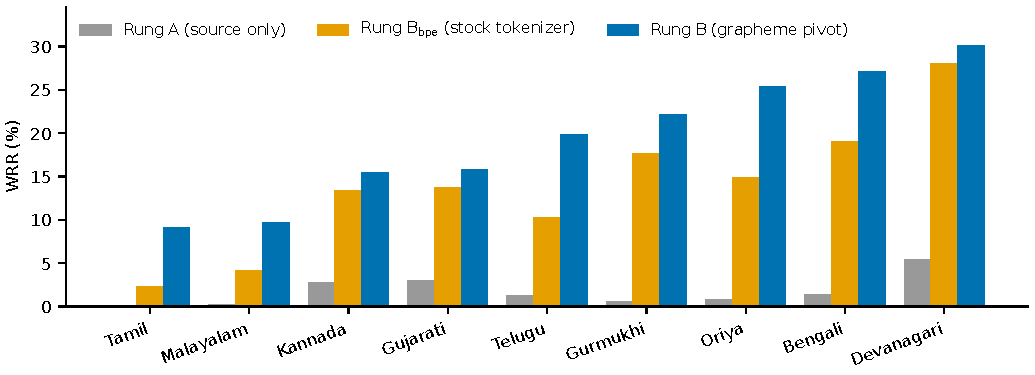
\includegraphics[width=\linewidth]{figs/fig2_bars.pdf}
  \caption{Transfer by script (ascending by Rung~B). Source-only baselines (grey) sit near the
  floor; the grapheme pivot (blue) beats the stock-BPE tokenizer (orange) on every one of the nine
  scripts under identical data and seed. Generated from the result JSONs by
  \texttt{make\_wacv\_figs.py}.}
  \label{fig:bars}
\end{figure}

\subsection{The pivot is the mechanism: BPE ablation}
\label{sec:ablation}

Removing the grapheme-cluster vocabulary --- same pivot strings, same images, same seed ---
degrades all nine scripts (Table~\ref{tab:main}), from $\bpeRatioMin\times$ (Devanagari,
\wrrBdevanagari\ $\rightarrow$ \wrrPdevanagari\ WRR) to $\bpeRatioMax\times$ (Tamil,
\wrrBtamil\ $\rightarrow$ \wrrPtamil): the margin varies, the direction never does (exact
two-sided sign test, $p=\bpeSignP$). The bootstrap makes the per-script margin concrete: on
\bpeCIdisjoint\ of nine the Rung-B 95\% CI clears the B$_{\mathrm{bpe}}$ interval outright
(Table~\ref{tab:main}); the three exceptions --- Devanagari, Kannada, Gujarati --- are exactly the
near-parity scripts ($\bpeRatioMin$--$1.16\times$), consistent with the direction holding but the
magnitude shrinking as fertility falls. The character-accuracy pattern is diagnostic: on Telugu
the BPE model \emph{matches} the pivot model's character accuracy (\chaPtelugu\% vs.\
\chaBtelugu\%), and on Kannada and Devanagari slightly exceeds it, yet word accuracy drops in
every case. Synthetic fine-tuning alone teaches the model to see the characters; the
cluster-level output space is what assembles them into correct whole words. The margin itself
is not noise: it grows with the held-out script's fertility, largest exactly on the
high-fertility Dravidian scripts where transfer is hardest
(Sec.~\ref{sec:fertility-fails}).

\subsection{Dose--response: synthetic budget}
\label{sec:scaling}

We hold the recipe fixed and vary only the number of synthetic target images, for the three
scripts whose held-out budget we can grow --- Malayalam, Kannada, Telugu --- across
$\{810, 1620, 6480, 12960\}$ renderings; the external Rung-B point (3240) anchors each curve.
Word recognition is cleanly log-linear in synthetic exposure ($R^2$ from \scaleRtwoMin\ to
\scaleRtwoMax\ per script), and the slope is \emph{script-invariant}: a single shared
$\scaleSlope$ WRR per doubling fits all three, with no evidence of differing slopes ($F$-test
$p=\scaleFp$; Fig.~\ref{fig:scaling}). This is the preregistered \emph{form}, and it holds.

The preregistered \emph{magnitude} does not. The frozen instrument projected
$+\tfTwoxBonus$ WRR per doubling --- transported from the in-script $2\times$-synthetic experiment
that fit the two-factor model (Sec.~\ref{sec:analysis}) --- which the swept slope excludes by a
factor of $\scaleSlopeRatio$: the faithful doubling step ($3240\!\rightarrow\!6480$) gained
$\scaleFaithfulObs$ WRR on average against a predicted $\scaleFaithfulPred$, a miss outside the
$\pm2$\,RMSE band and reported as filed (open squares, Fig.~\ref{fig:scaling}). Two further
preregistered edges resolve the same way. The low-budget prediction of near-collapse toward the
Rung-A floor is \emph{falsified} --- Kannada and Telugu already reach double digits at 810 images,
so transfer is concave, not linear, in log-budget --- while the top step
($6480\!\rightarrow\!12960$), which adds renderings at near-fixed lexicon, gains little on Kannada
(onset of lexicon saturation) but keeps pace on Malayalam and Telugu. Synthetic scaling is thus
real and orderly, but far shallower than an in-script extrapolation predicts; we report the
confirmed form and the missed coefficient together. We do \emph{not} promote pivot-space coverage
to a cross-script driver: it orders the three swept scripts in-sample, but across the six scripts
never used in the fit it is uncorrelated with transfer ($r=\covOOSr$), so the coverage axis (three
distinct values) is underdetermined and we disclose it rather than build on it.

\begin{figure}[t]
  \centering
  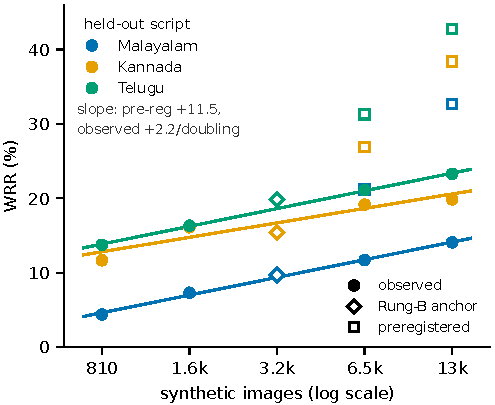
\includegraphics{figs/fig3_scaling.pdf}
  \caption{Synthetic-budget dose--response for three held-out scripts. Filled circles: observed WRR
  on real test images; solid lines: per-script log-linear fits (shared slope
  $\scaleSlope$/doubling). Open diamonds: the external Rung-B anchor (3240 images). Open squares:
  the preregistered point predictions --- their gap above the observed points is the
  $\scaleSlopeRatio\times$ magnitude miss, reported as filed.}
  \label{fig:scaling}
\end{figure}

\subsection{Out-of-benchmark: Khmer}
\label{sec:khmer}

\TODO{Preregistered Amendment 4b: train on all nine benchmark scripts + synthetic Khmer
(different Unicode block, coeng-based stacking, outside the benchmark and outside India);
evaluate on KhmerST~\cite{khmerst}. PROSPECTIVE\_PREDICTION\_KHMER filed from the frozen
two-factor model before training. Timeboxed; paper stands without it if the segmenter/crop
engineering misses the freeze date.}

\subsection{Frontier-VLM reference}
\label{sec:vlm}

We prompt Qwen2.5-VL-7B~\cite{qwen25vl} zero-shot on the same nine real test sets (fixed prompt,
greedy decoding), preregistered under Amendment~4c. Under the declared primary metric --- exact
word match on the raw generation, our shared normalization --- it scores $0.0\%$ on all nine: the
chat model wraps every answer in prose (``The text in the image is~\dots''). We therefore report a
\emph{disclosed, most-favourable} re-score (Table~\ref{tab:vlm}): we extract the first quoted span
from each generation and apply the identical metric. Even so, the VLM reads only the two
highest-resource scripts with any competence --- Bengali \vlmWrrBengali\% and Devanagari
\vlmWrrDevanagari\% --- and is at or near zero on six of the remaining seven (at most
\vlmWrrTamil\%, on Tamil), frequently transcribing a wholly different script (Gurmukhi returned in
Devanagari, Malayalam in Bengali). Our compact pivot model, at a fraction of the parameters, wins
on \vlmScriptsWon\ of nine, the VLM leading only on Devanagari, the single most-resourced Indic
script. The comparison is not like-for-like --- the VLM's training data is unknown and it is an
upper-bound reference for off-the-shelf capability, not a system built for this task --- but it
establishes that scale alone does not read these scripts; frontier models cover fewer than thirty
of 100+ writing systems~\cite{glotocr}.

\begin{table}[t]
  \centering\small
  \setlength{\tabcolsep}{6pt}
  \begin{tabular}{lrr}
    \toprule
    Script & Ours (Rung~B) & Qwen2.5-VL-7B \\
    \midrule
    Tamil      & \textbf{\wrrBtamil}      & \vlmWrrTamil      \\
    Telugu     & \textbf{\wrrBtelugu}     & \vlmWrrTelugu     \\
    Kannada    & \textbf{\wrrBkannada}    & \vlmWrrKannada    \\
    Malayalam  & \textbf{\wrrBmalayalam}  & \vlmWrrMalayalam  \\
    Oriya      & \textbf{\wrrBoriya}      & \vlmWrrOriya      \\
    Gujarati   & \textbf{\wrrBgujarati}   & \vlmWrrGujarati   \\
    Bengali    & \textbf{\wrrBbengali}    & \vlmWrrBengali    \\
    Devanagari & \wrrBdevanagari          & \textbf{\vlmWrrDevanagari} \\
    Gurmukhi   & \textbf{\wrrBgurmukhi}   & \vlmWrrGurmukhi   \\
    \midrule
    macro avg  & --                       & \vlmMacro         \\
    \bottomrule
  \end{tabular}
  \caption{Zero-shot WRR (\%) vs.\ a frontier VLM on the same real test images. Qwen2.5-VL scored
  under a disclosed, most-favourable extraction (its preregistered exact-match primary is $0.0$ on
  all nine). Our compact model wins on \vlmScriptsWon\ of nine; the VLM leads only on Devanagari,
  the most-resourced Indic script.}
  \label{tab:vlm}
\end{table}
